% https://tex.stackexchange.com/questions/64836/change-image-size#64843
%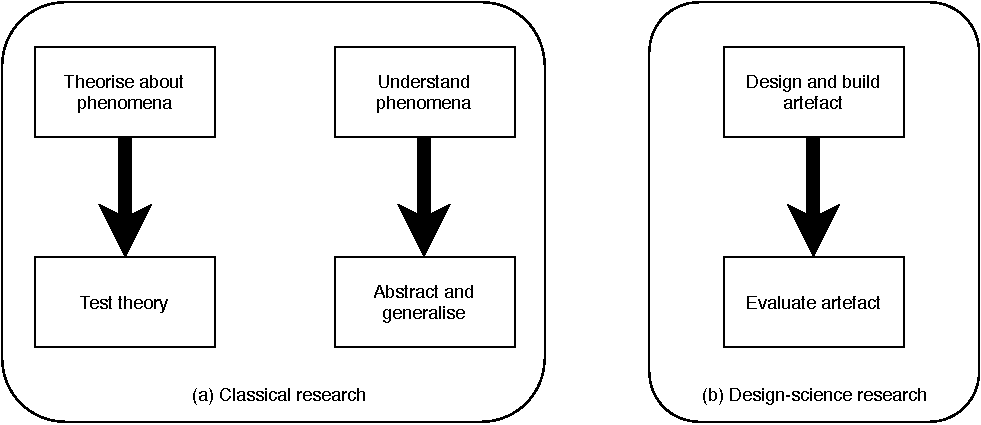
\includegraphics[width=0.9\columnwidth]{TypesOfResearch.pdf}
\begin{figure}[!htb]
    \caption{Diastolic Blood Pressure Membership}
    \[
        \textit{DBP}_{normal}(q) = \left\{%
        \begin{array}{ll}
            1                  & \textrm{if }q<60,       \\
            \frac{60-q}{80-60} & \textrm{if }60\ge q<80. \\
        \end{array}%
        \right.
    \]

    \[
        \textit{DBP}_{high}(q) = \left\{%
        \begin{array}{ll}
            \frac{117-q}{85} & \textrm{if }90\ge q<100, \\
            1                & \textrm{if }\ge 100.     \\
        \end{array}%
        \right.
    \]
    \label{fig:diastolic}
\end{figure}
